\fhooelecture[Global Acting in IT]{\Huge International Minor: Global Acting in IT}{International Minor: Global Acting in IT}{GAIT}

\begin{frame}{International Minor: Global Acting in IT}
\begin{center}%
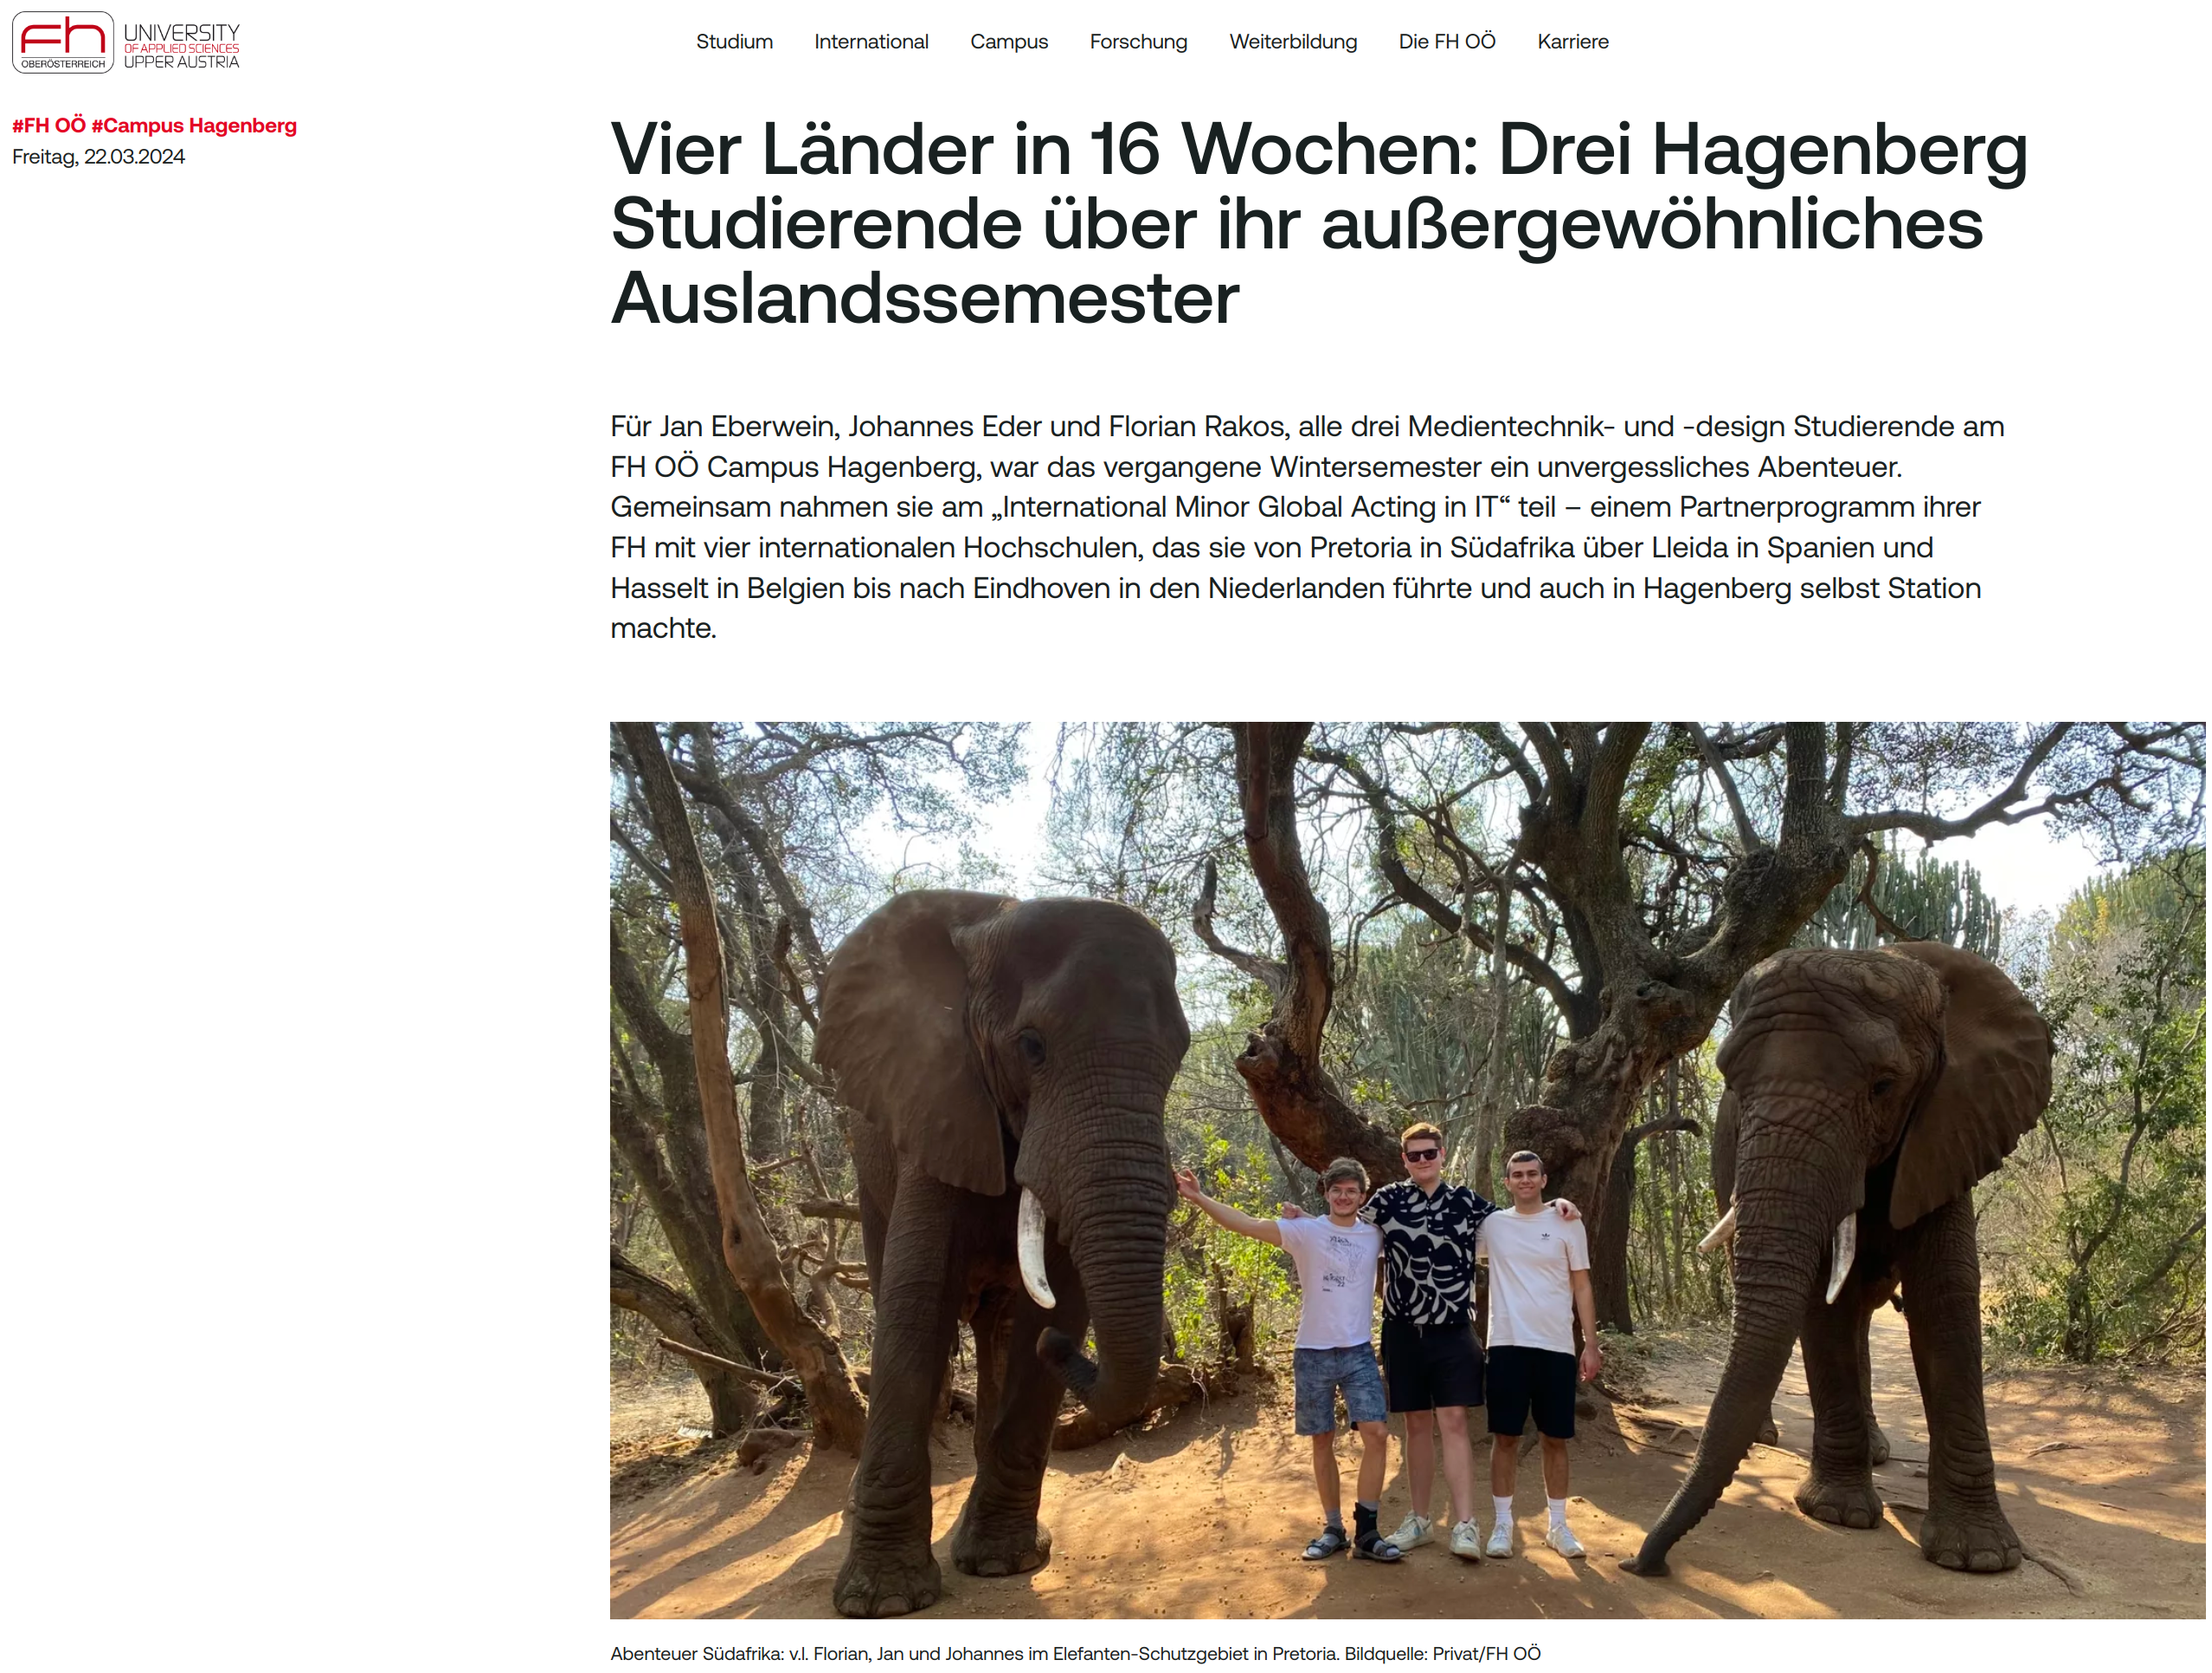
\includegraphics[width=0.65\textwidth]{material/international-minor.png}%
\end{center}
\end{frame}

\begin{frame}{International Minor: Global Acting in IT – Struktur}
\centering Angesiedelt im fünften Semester des Bachelorstudiengangs Medientechnik und Design%
\begin{center}%

\includegraphics[width=0.74\textwidth]{material/Global-Acting-in-ICT-2024-2.png}%
\vspace{0.5cm}\\%
\LARGE Semesterübergreifendes Leitthema: \alert{Invasive Arten}
\end{center}
\end{frame}

\begin{frame}{Studierende des International Minor 2024}
    \begin{center}
        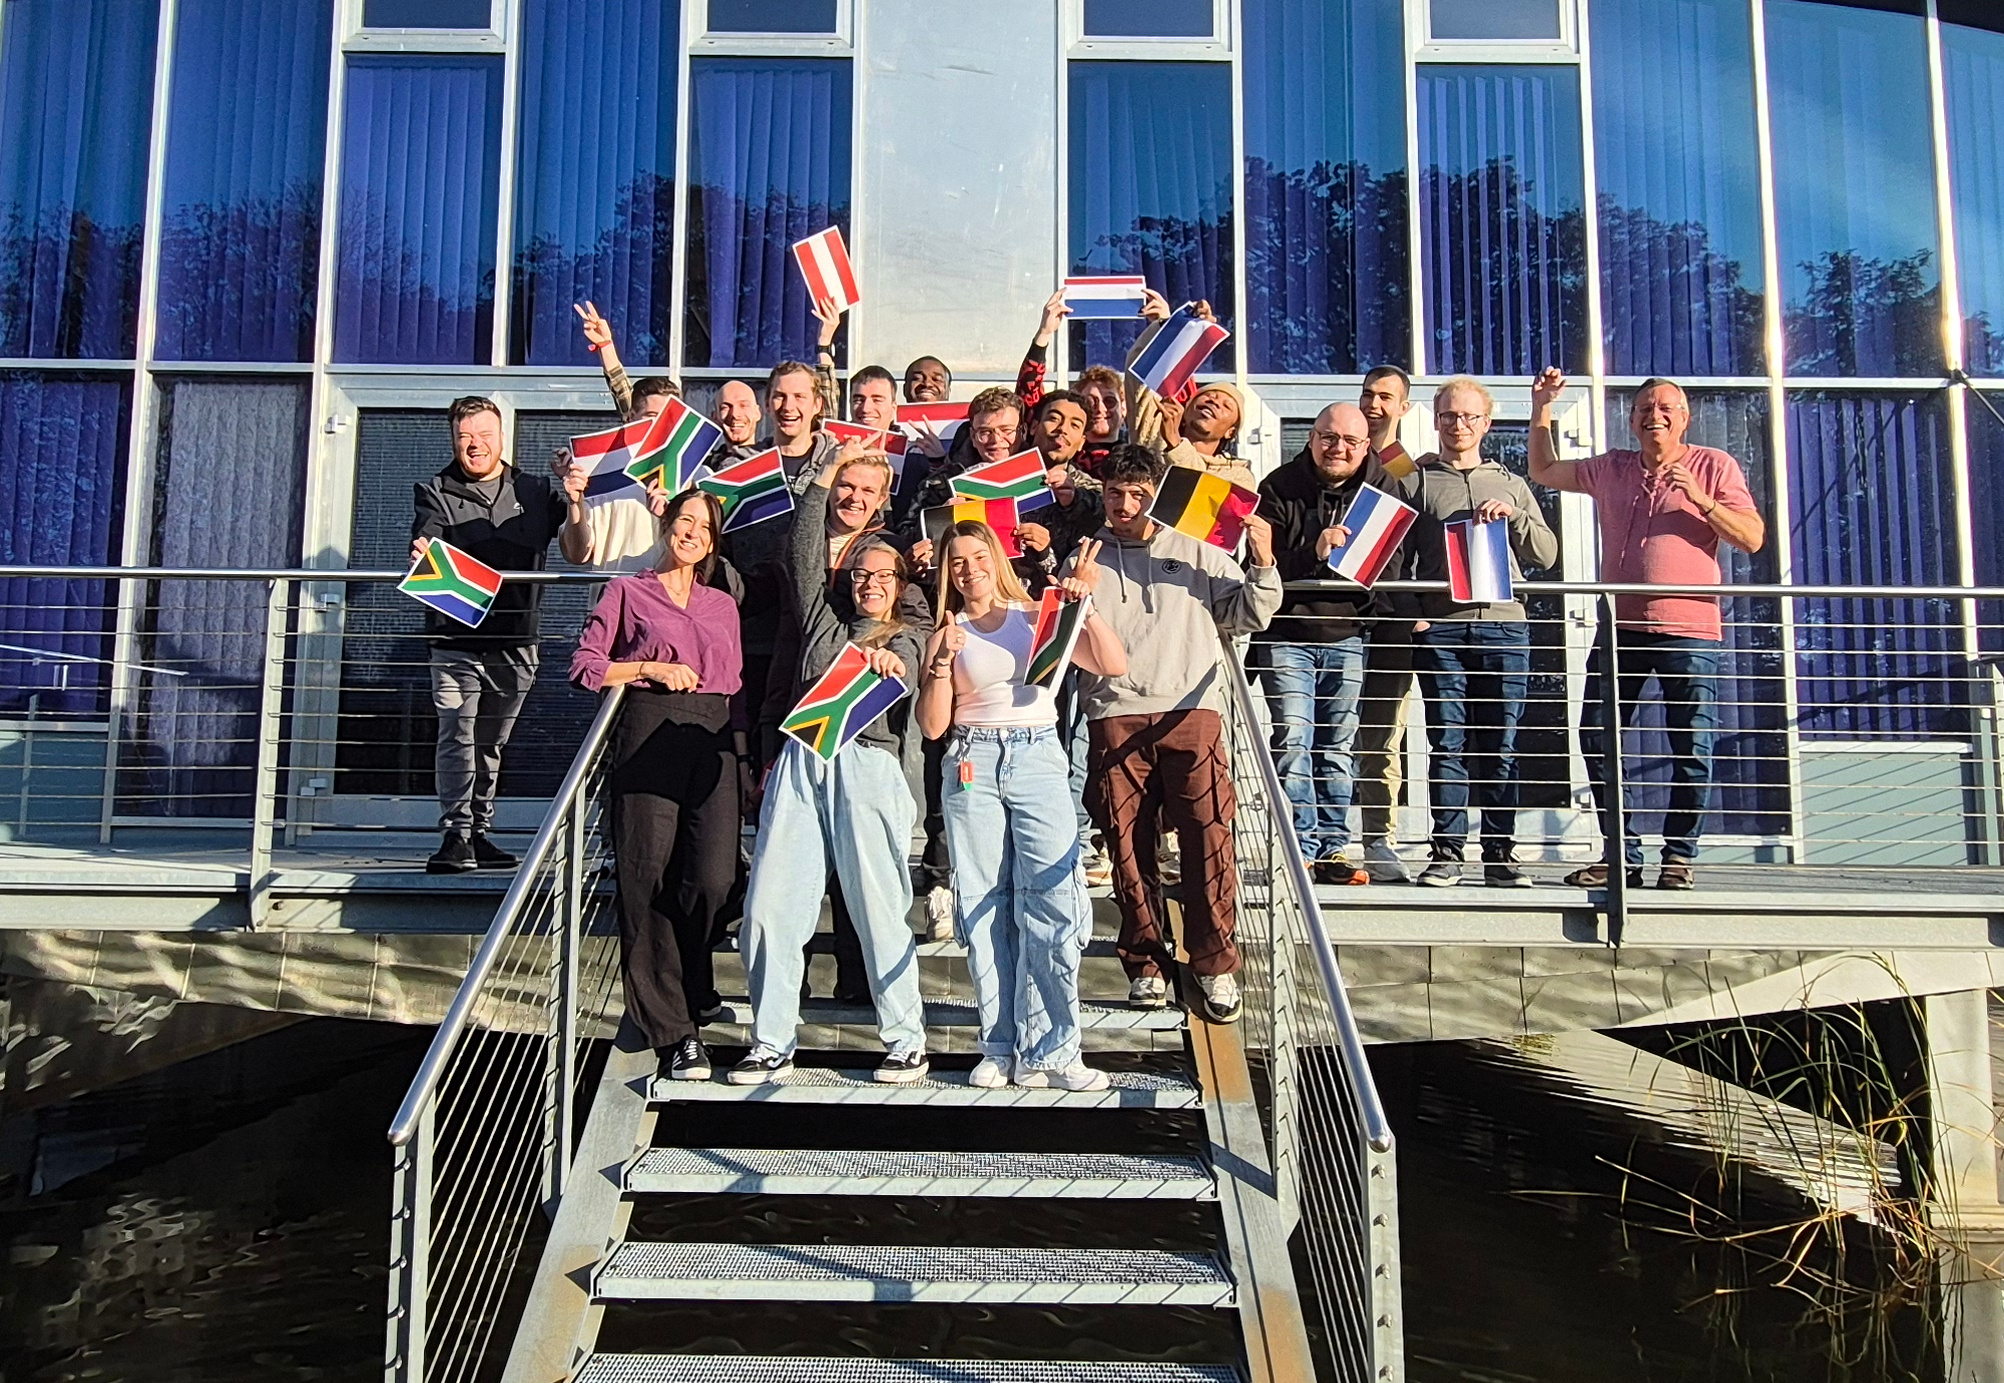
\includegraphics[width=0.73\textwidth]{material/InternationalMinorStudents2024.jpg}
    \end{center}
\end{frame}
%\nopartpage
\part{Die invasive Art Wasserhyazinthen}
%\withpartpage

\section[withsectionpage]{Bezug zum Projekt des \emph{Centre for Biological Control} (Rhodes University, ZA)}

\begin{frame}{Die \alert{invasive} Art \alert{Wasserhyazinthe} besiedelt den \alert{Hartbeespoort-Damm}}{Wasserhyazinthen sind in Südamerika heimisch}
{\centering \LARGE \textbf{Wasserhyazinthen sind nicht in Afrika heimisch}\\}
\medskip
Wie kann IoT \alert{Prof. Julie Coetzee} und das \alert{\emph{Centre for Biological Control}} (Rhodes University, Südafrika) in der Forschung unterstützen?
\begin{center}
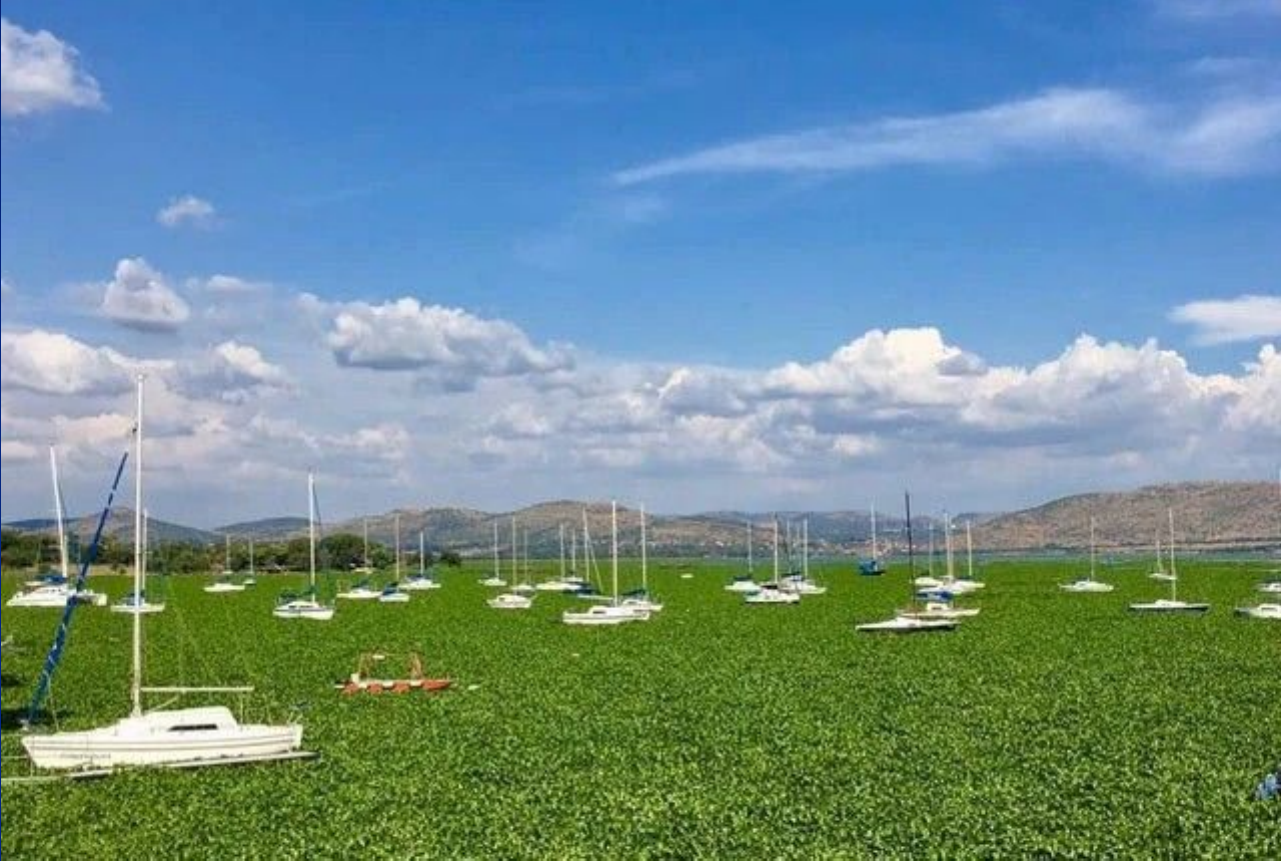
\includegraphics[width=0.53\textwidth]{material/Screenshot_20260125_034336}
\end{center}
\end{frame}

\begin{frame}{Lage des \alert{Hartbeespoort-Damms} (Pretoria)}{Wasserhyazinthen sind nicht in Afrika heimisch}
  \centering
  \makeatletter
\hspace*{-\dimexpr(\paperwidth-\textwidth-2.2em)/2\relax}%
  \hbox to \paperwidth{%
    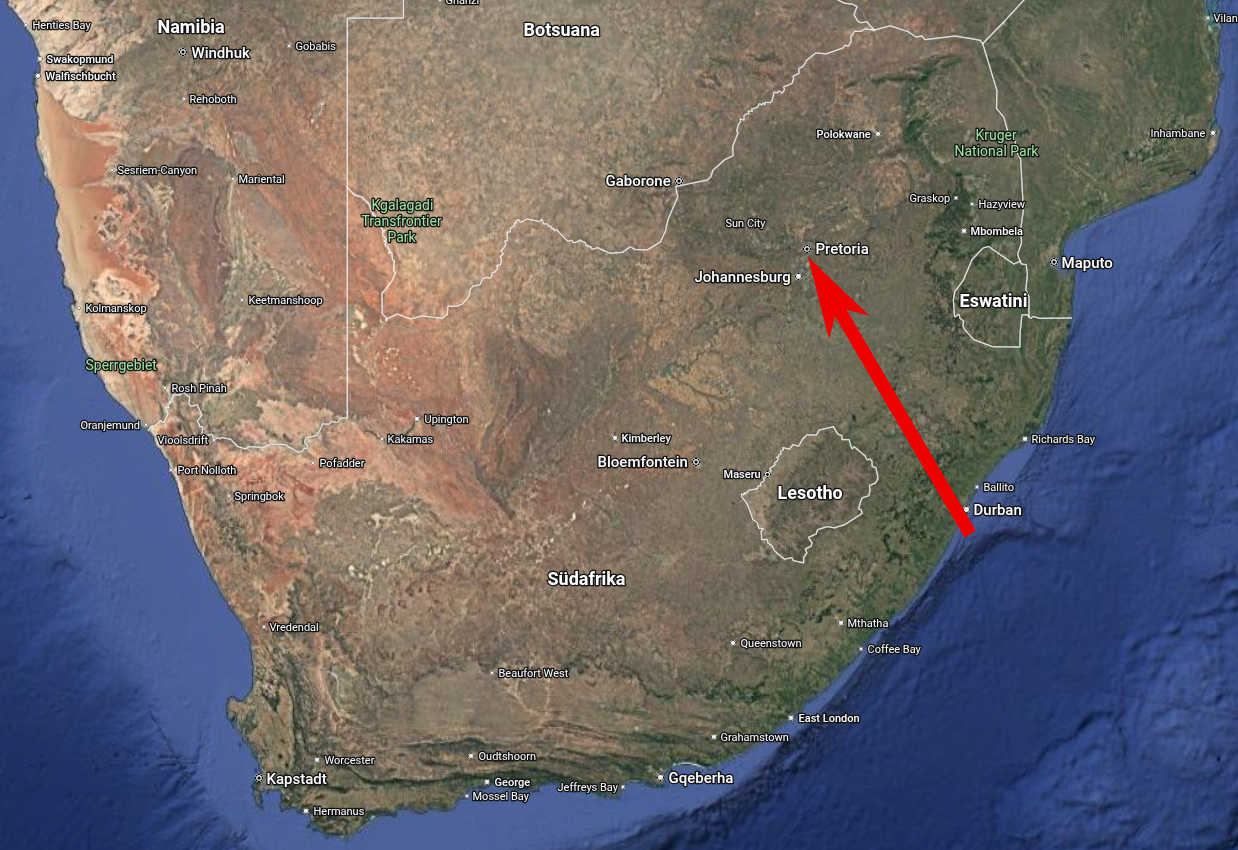
\includegraphics[width=.43\paperwidth]{material/Screenshot_20260125_045141-1}%
	\hfill
    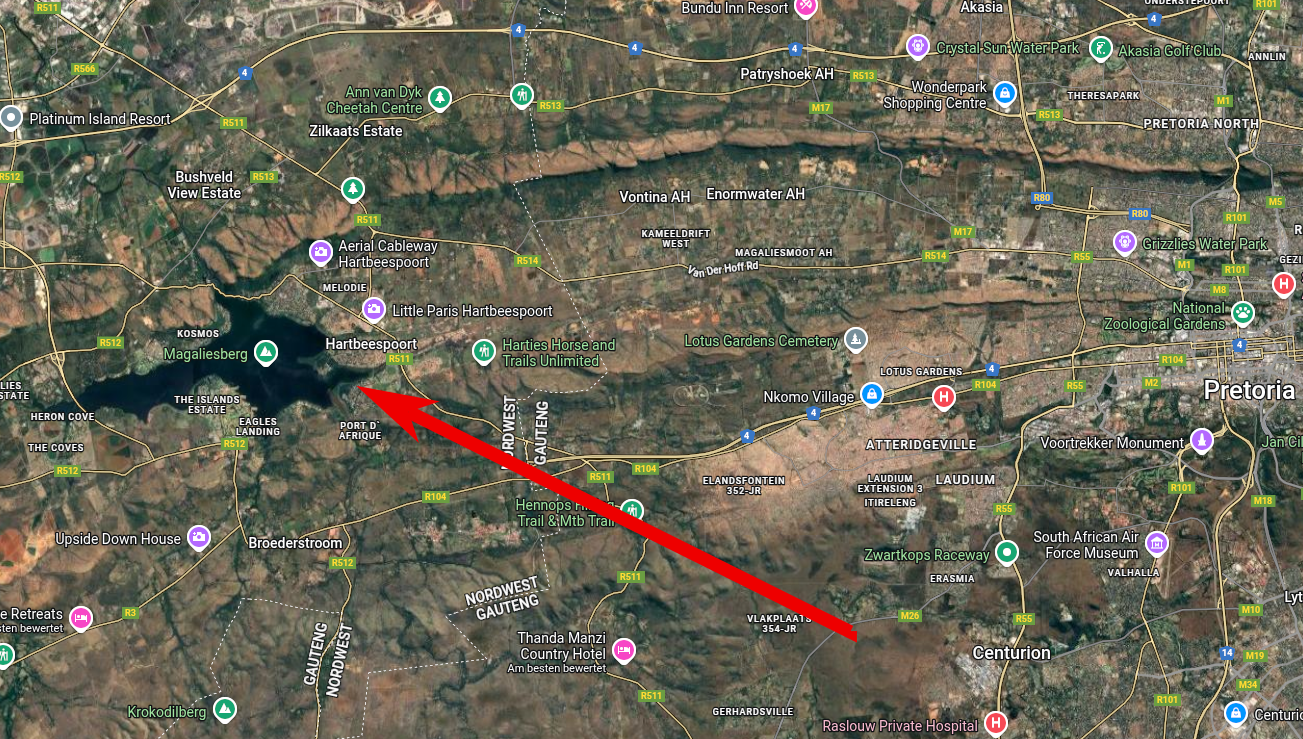
\includegraphics[width=.52\paperwidth]{material/Screenshot_20260125_045258-1}%
\hspace{1.5em}
  }%
  \makeatother
\end{frame}

\begin{frame}{Befall des Hartbeespoort-Damms durch Wasserhyazinthen}
	\only<1>{\centering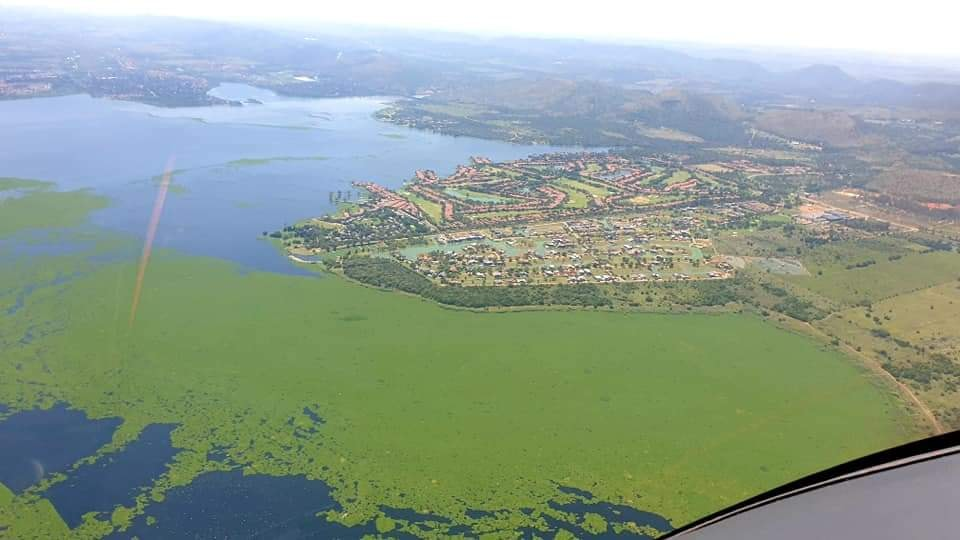
\includegraphics[width=0.85\textwidth]{material/481222896_29030362593228711_5940730522337148013_n}}%
	\only<2>{\centering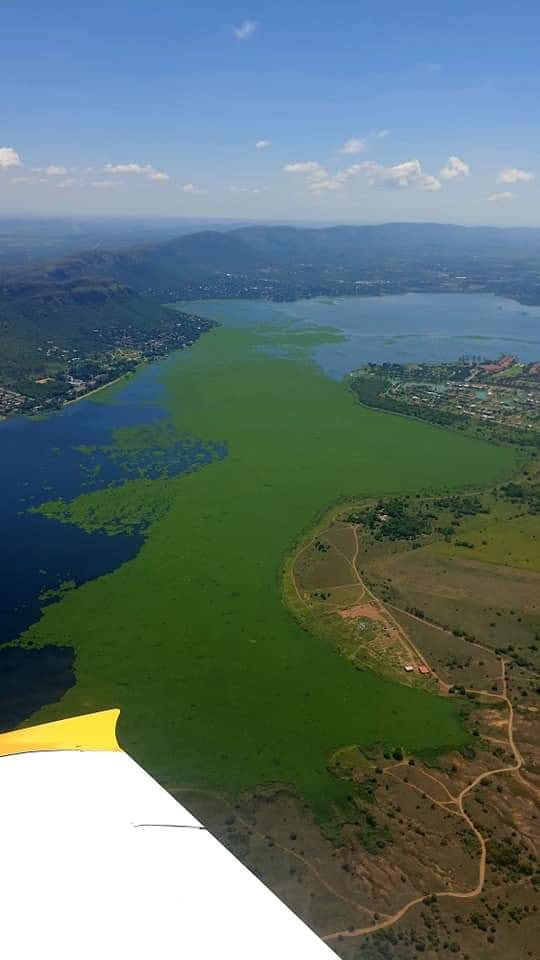
\includegraphics[height=0.86\textheight]{material/480709051_29030362869895350_5664085378424073827_n}\hspace{6em}\centering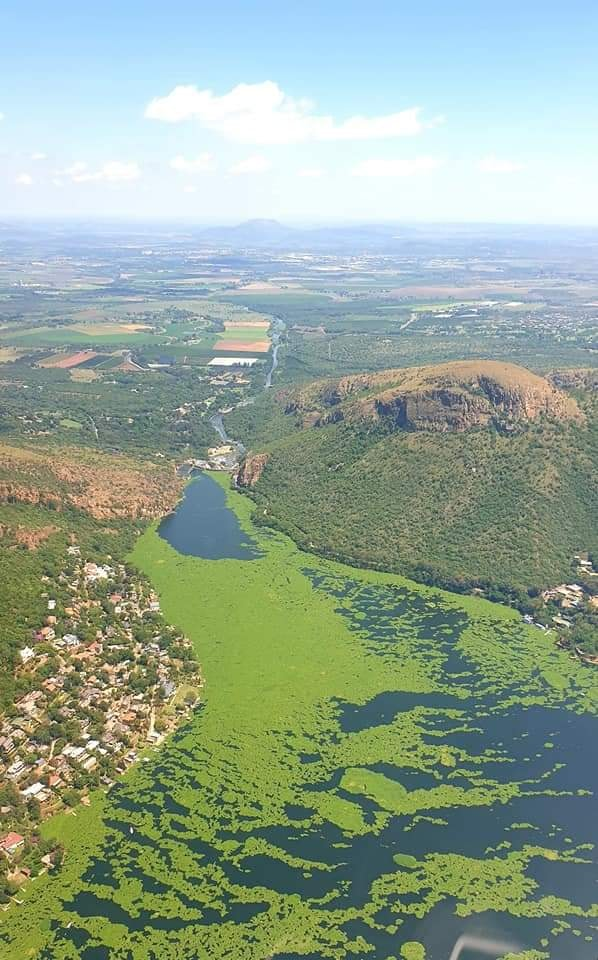
\includegraphics[height=0.86\textheight]{material/481654444_29030362819895355_3771374369220748004_n}}
\end{frame}

\begin{frame}{Weitere Fotos zur Veranschaulichung des Wasserhyazinthen-Befalls}
	\only<1>{\centering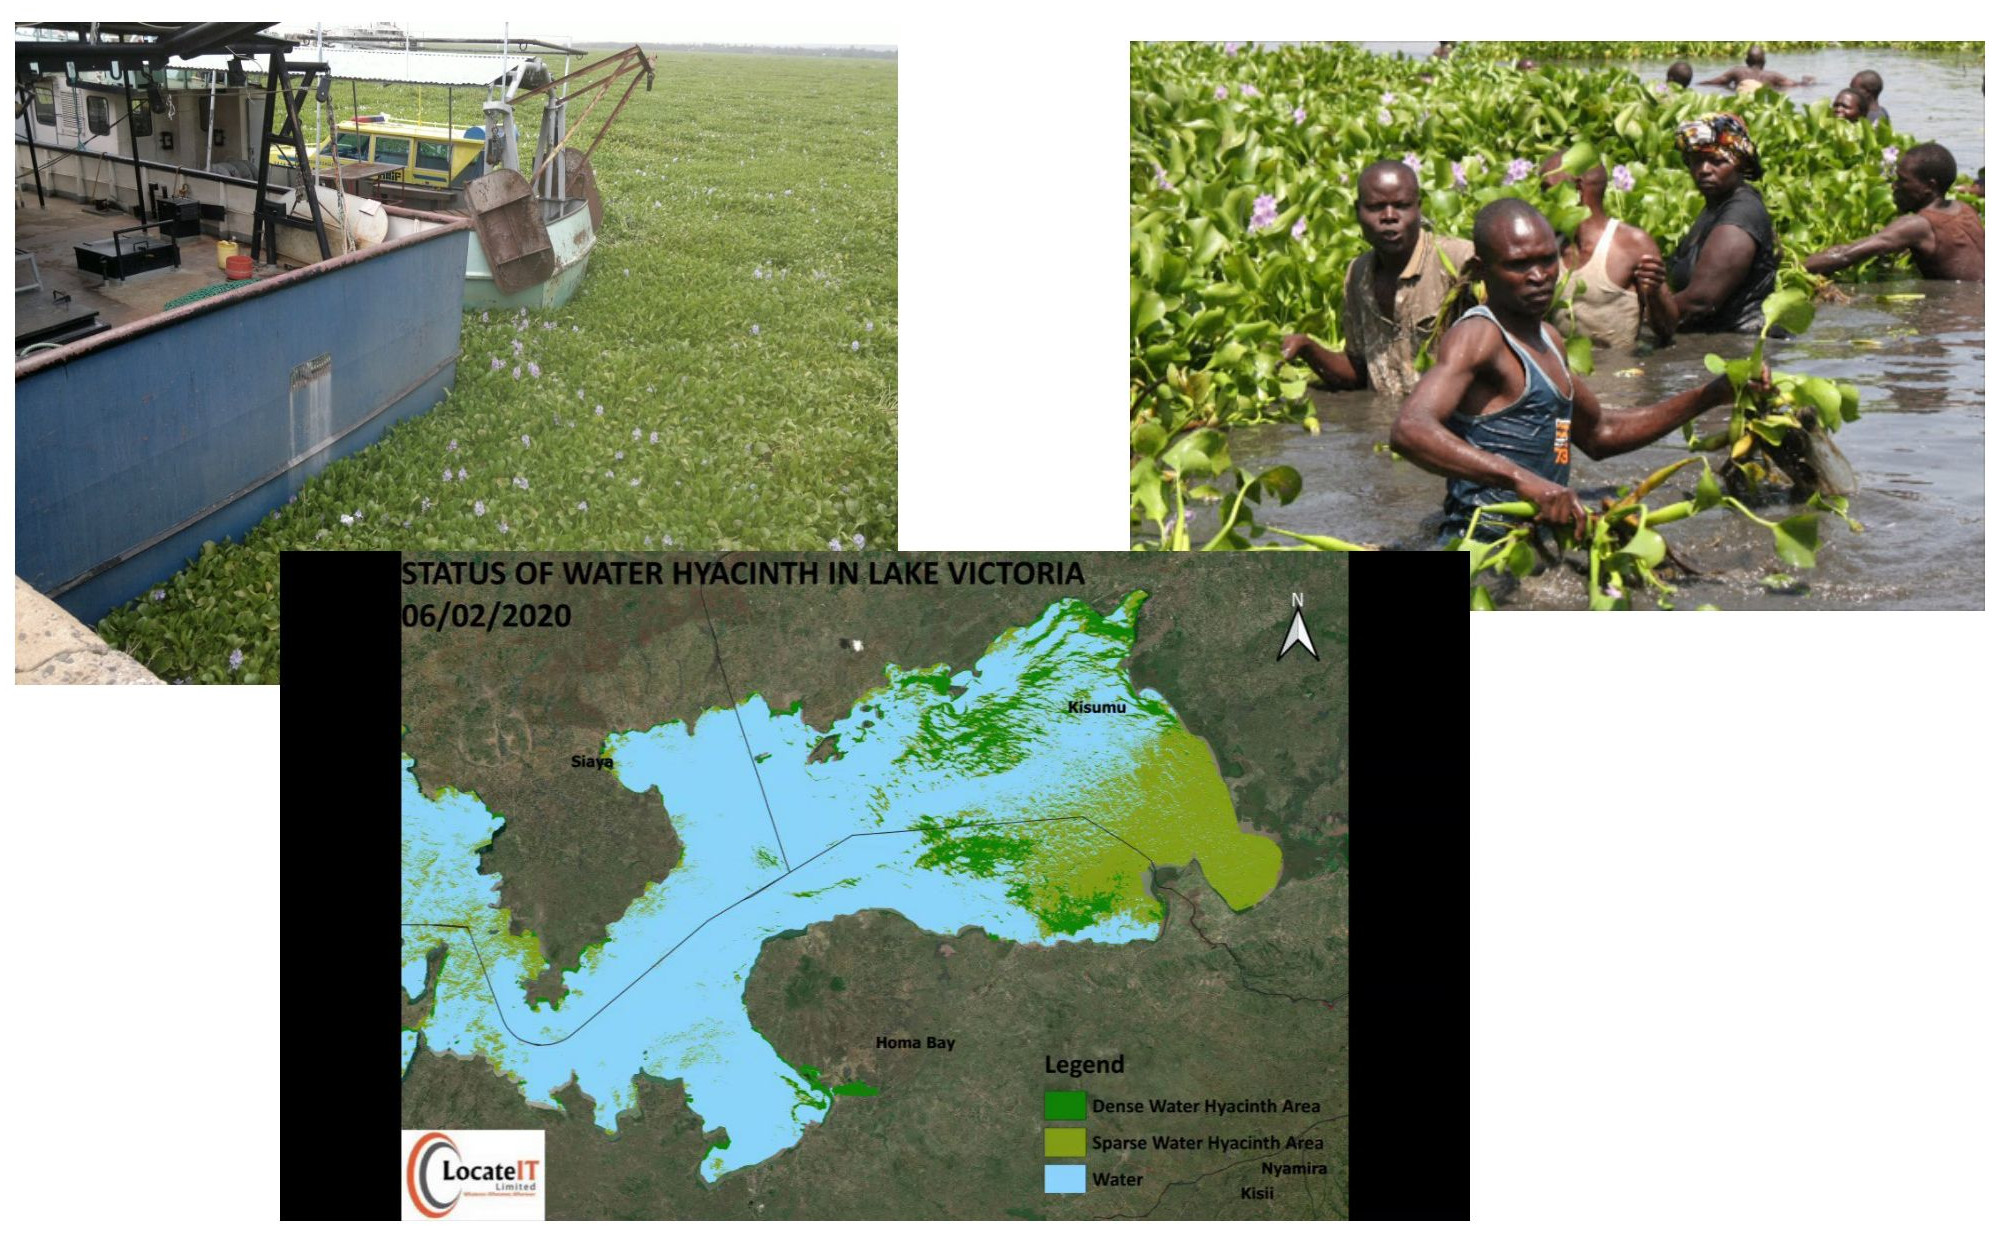
\includegraphics[width=0.85\textwidth]{material/water-hyacinth}}
	\only<2>{\centering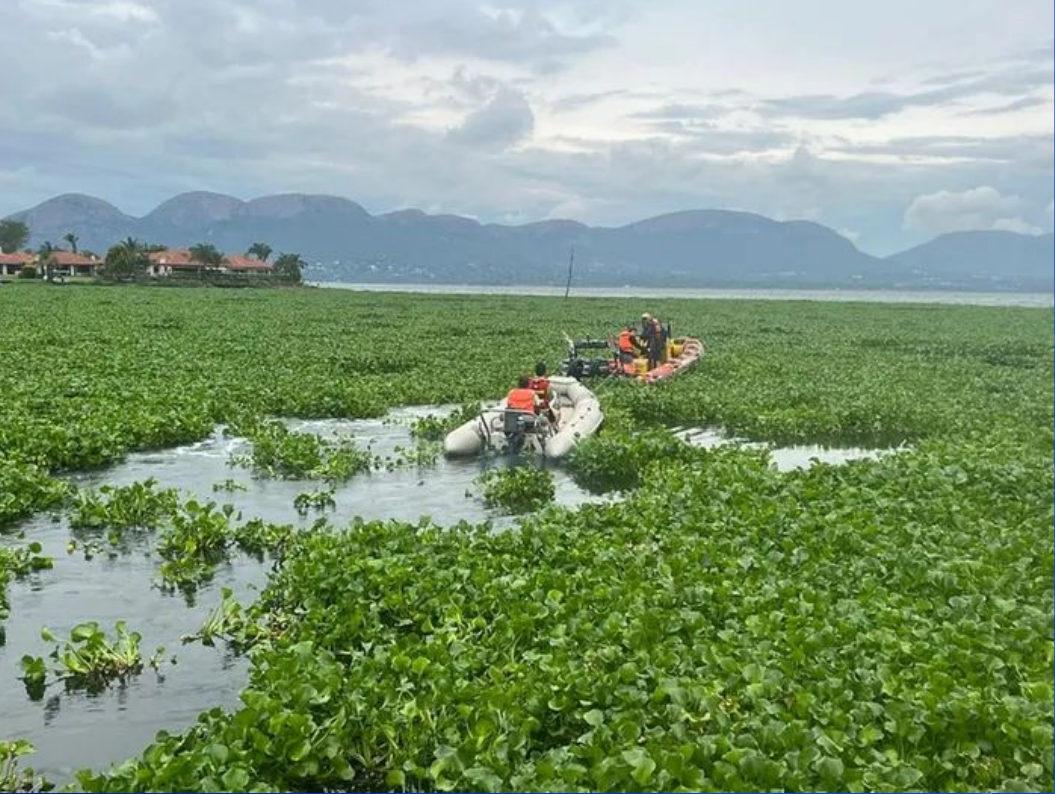
\includegraphics[width=0.68\textwidth]{material/Screenshot_20260125_041843}}
\end{frame}

\begin{frame}{Die Ausbreitung schwankt im Rhythmus der Jahreszeiten}
\only<1>{\centering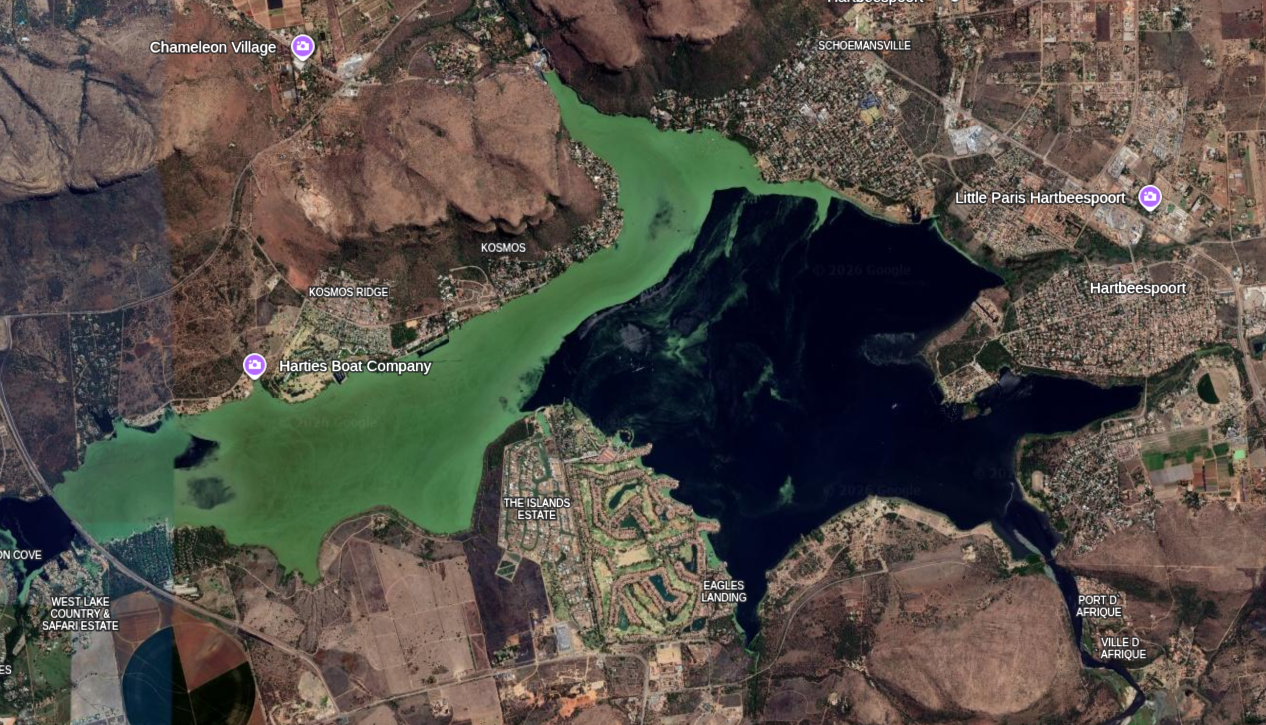
\includegraphics[width=0.84\textwidth]{material/Screenshot_20260125_044720}\\
\alert{Sommer}}
\only<2>{\centering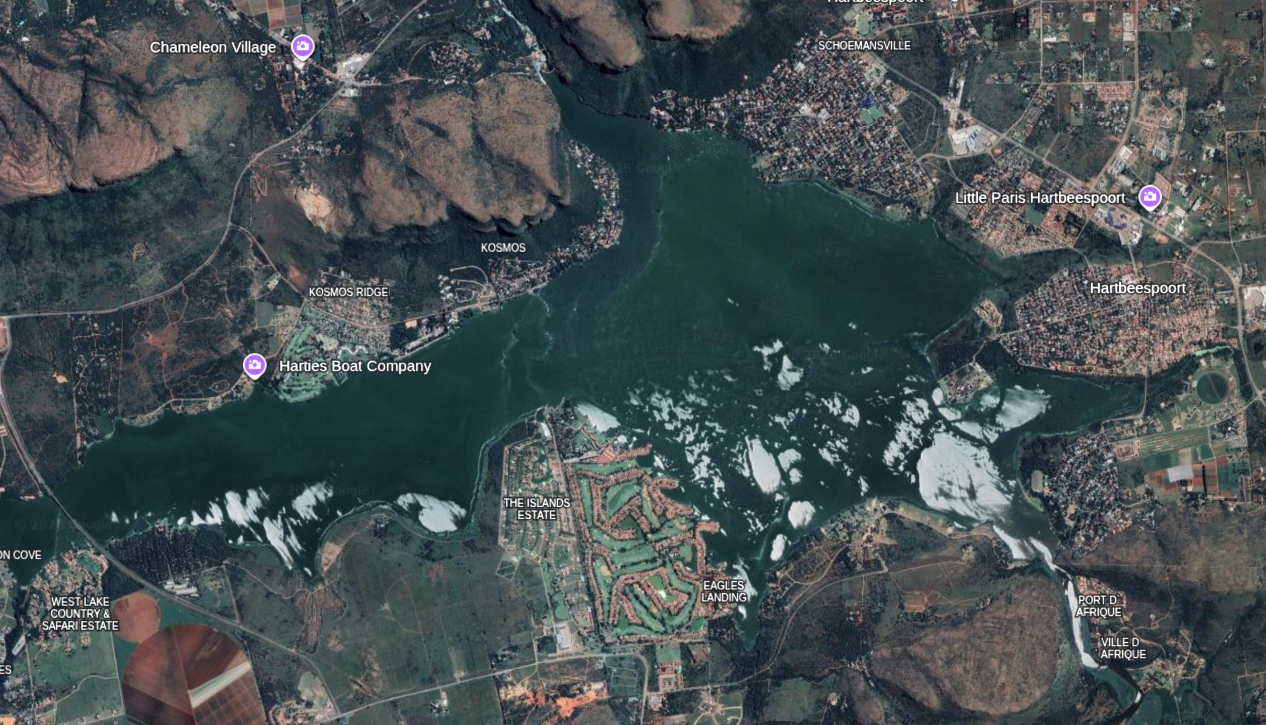
\includegraphics[width=0.84\textwidth]{material/Screenshot_20260125_044820}\\
\alert{Winter}}%
\end{frame}

\begin{frame}{Eines der Probleme: Wasserhyazinthen sind „schön“}
\only<1>{\centering{
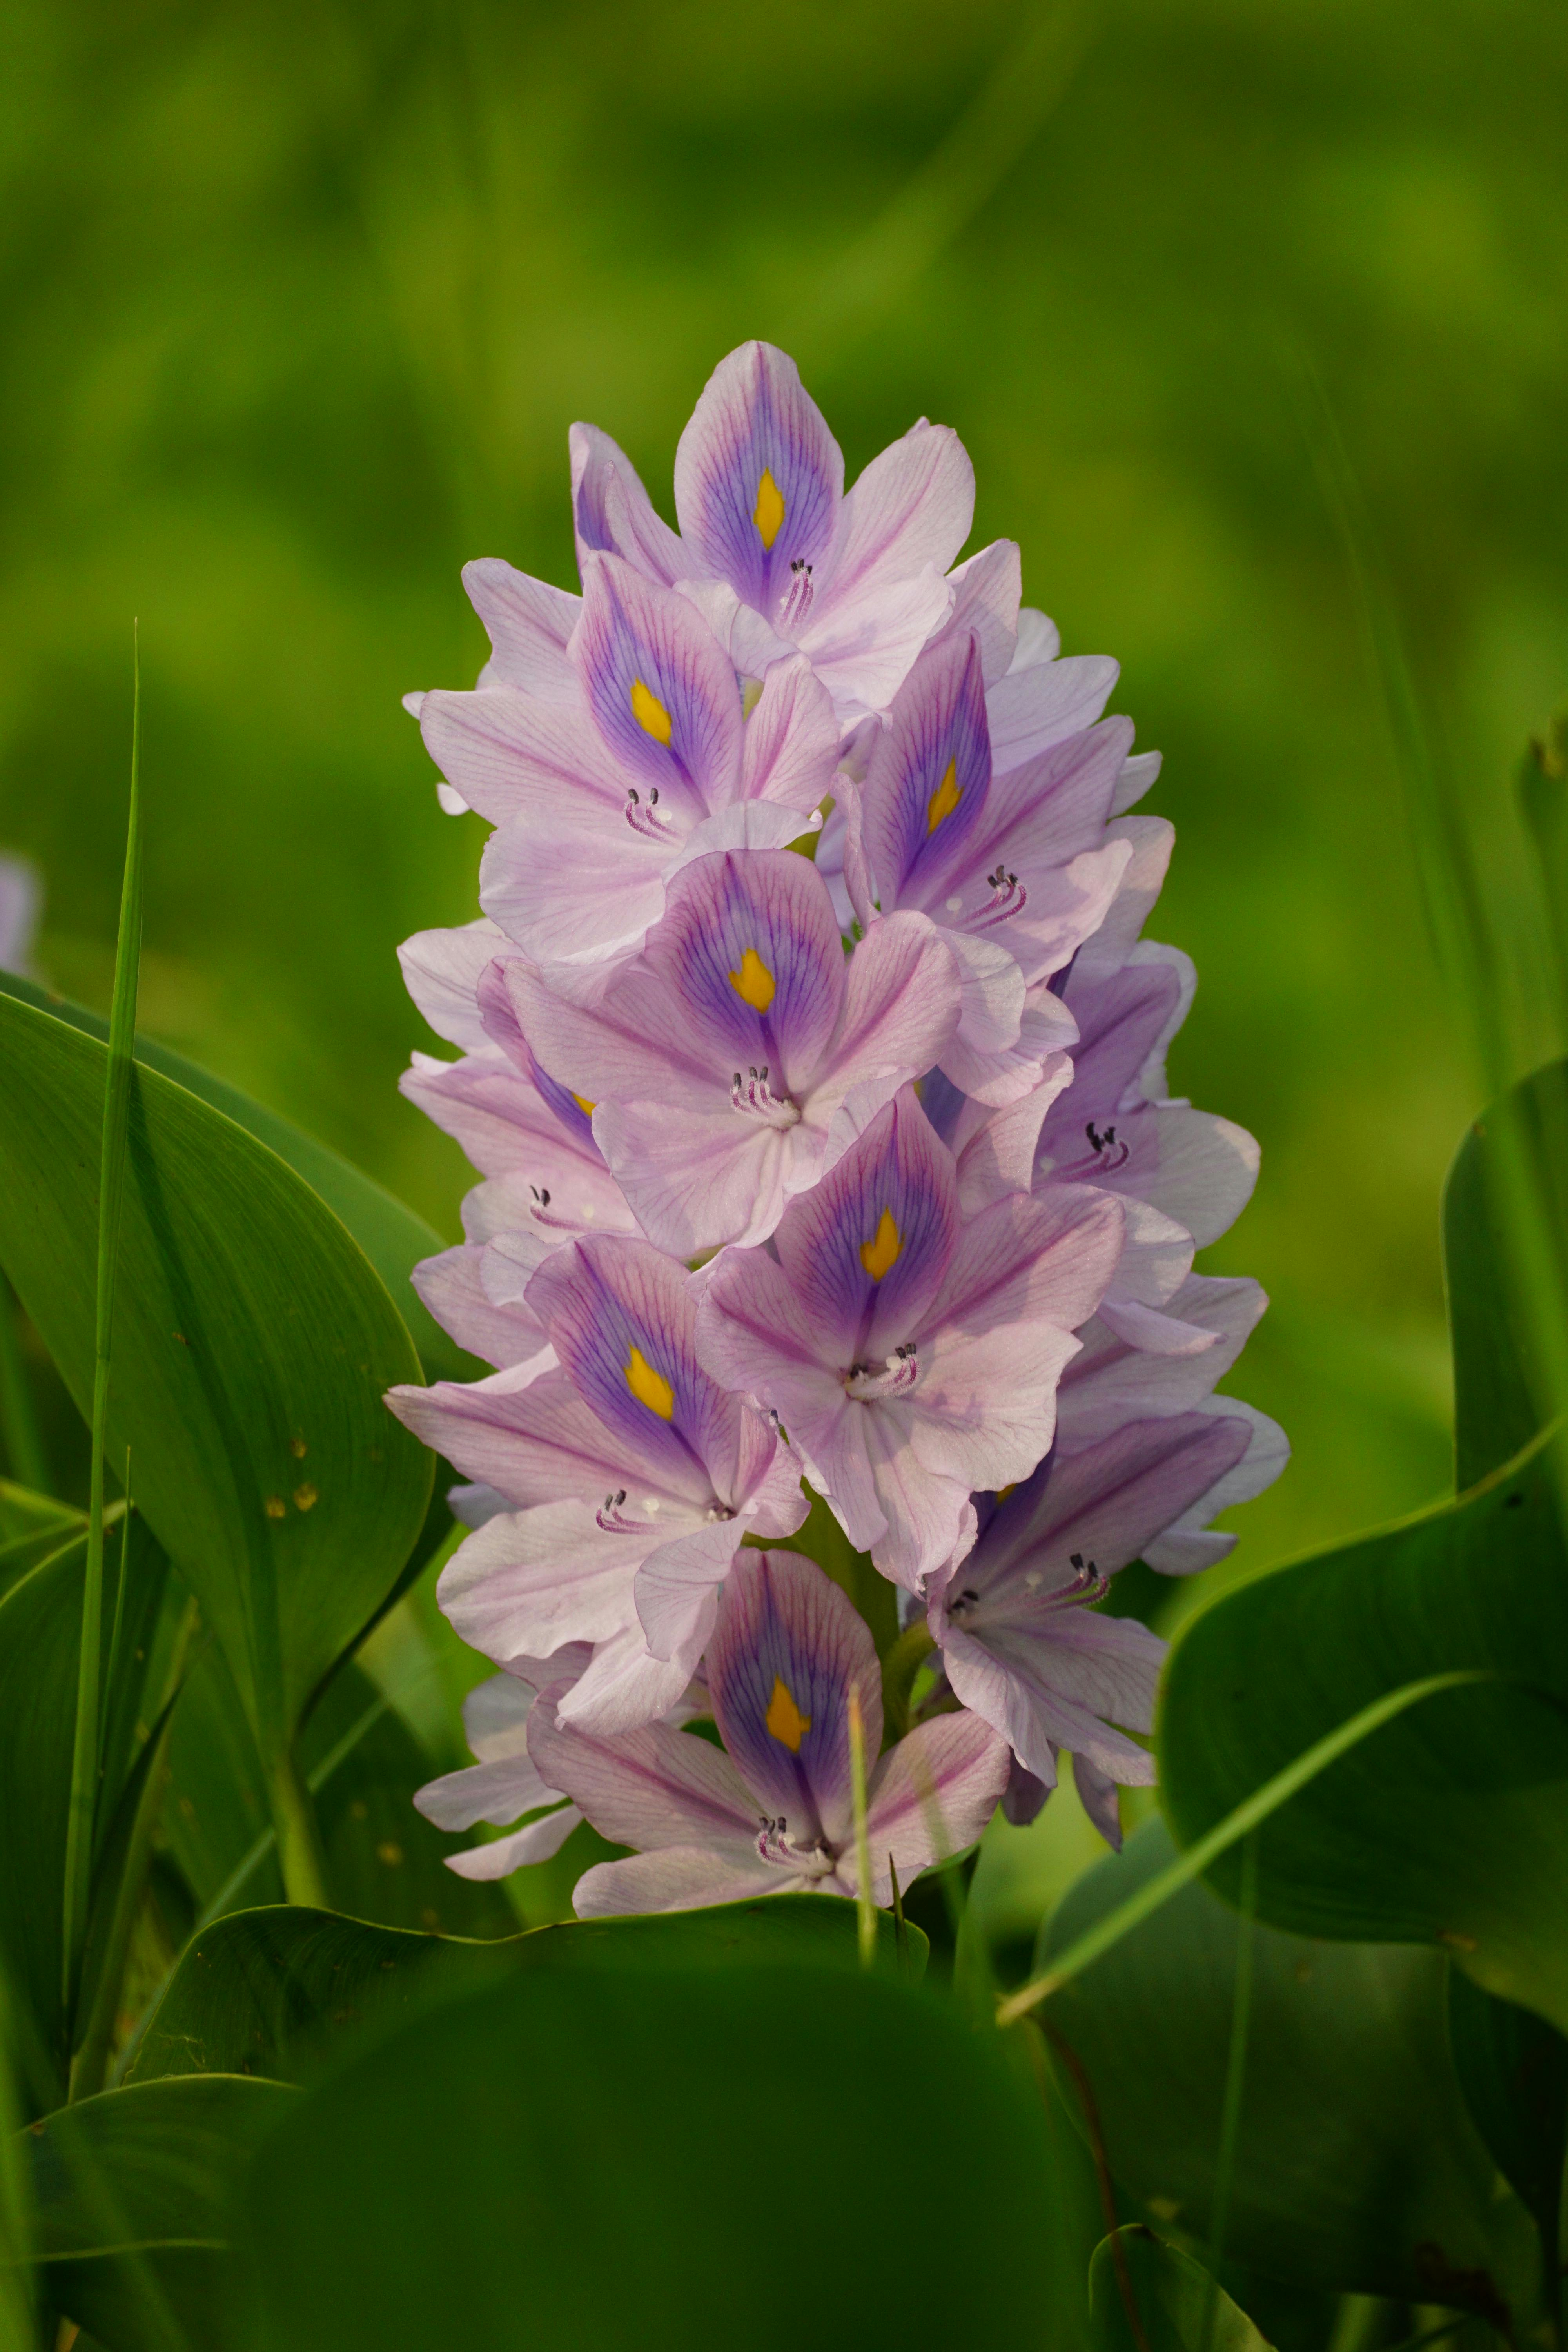
\includegraphics[height=0.85\textheight]{material/pexels-duy-le-duc-1257907900-23614068}
\hspace{5em}
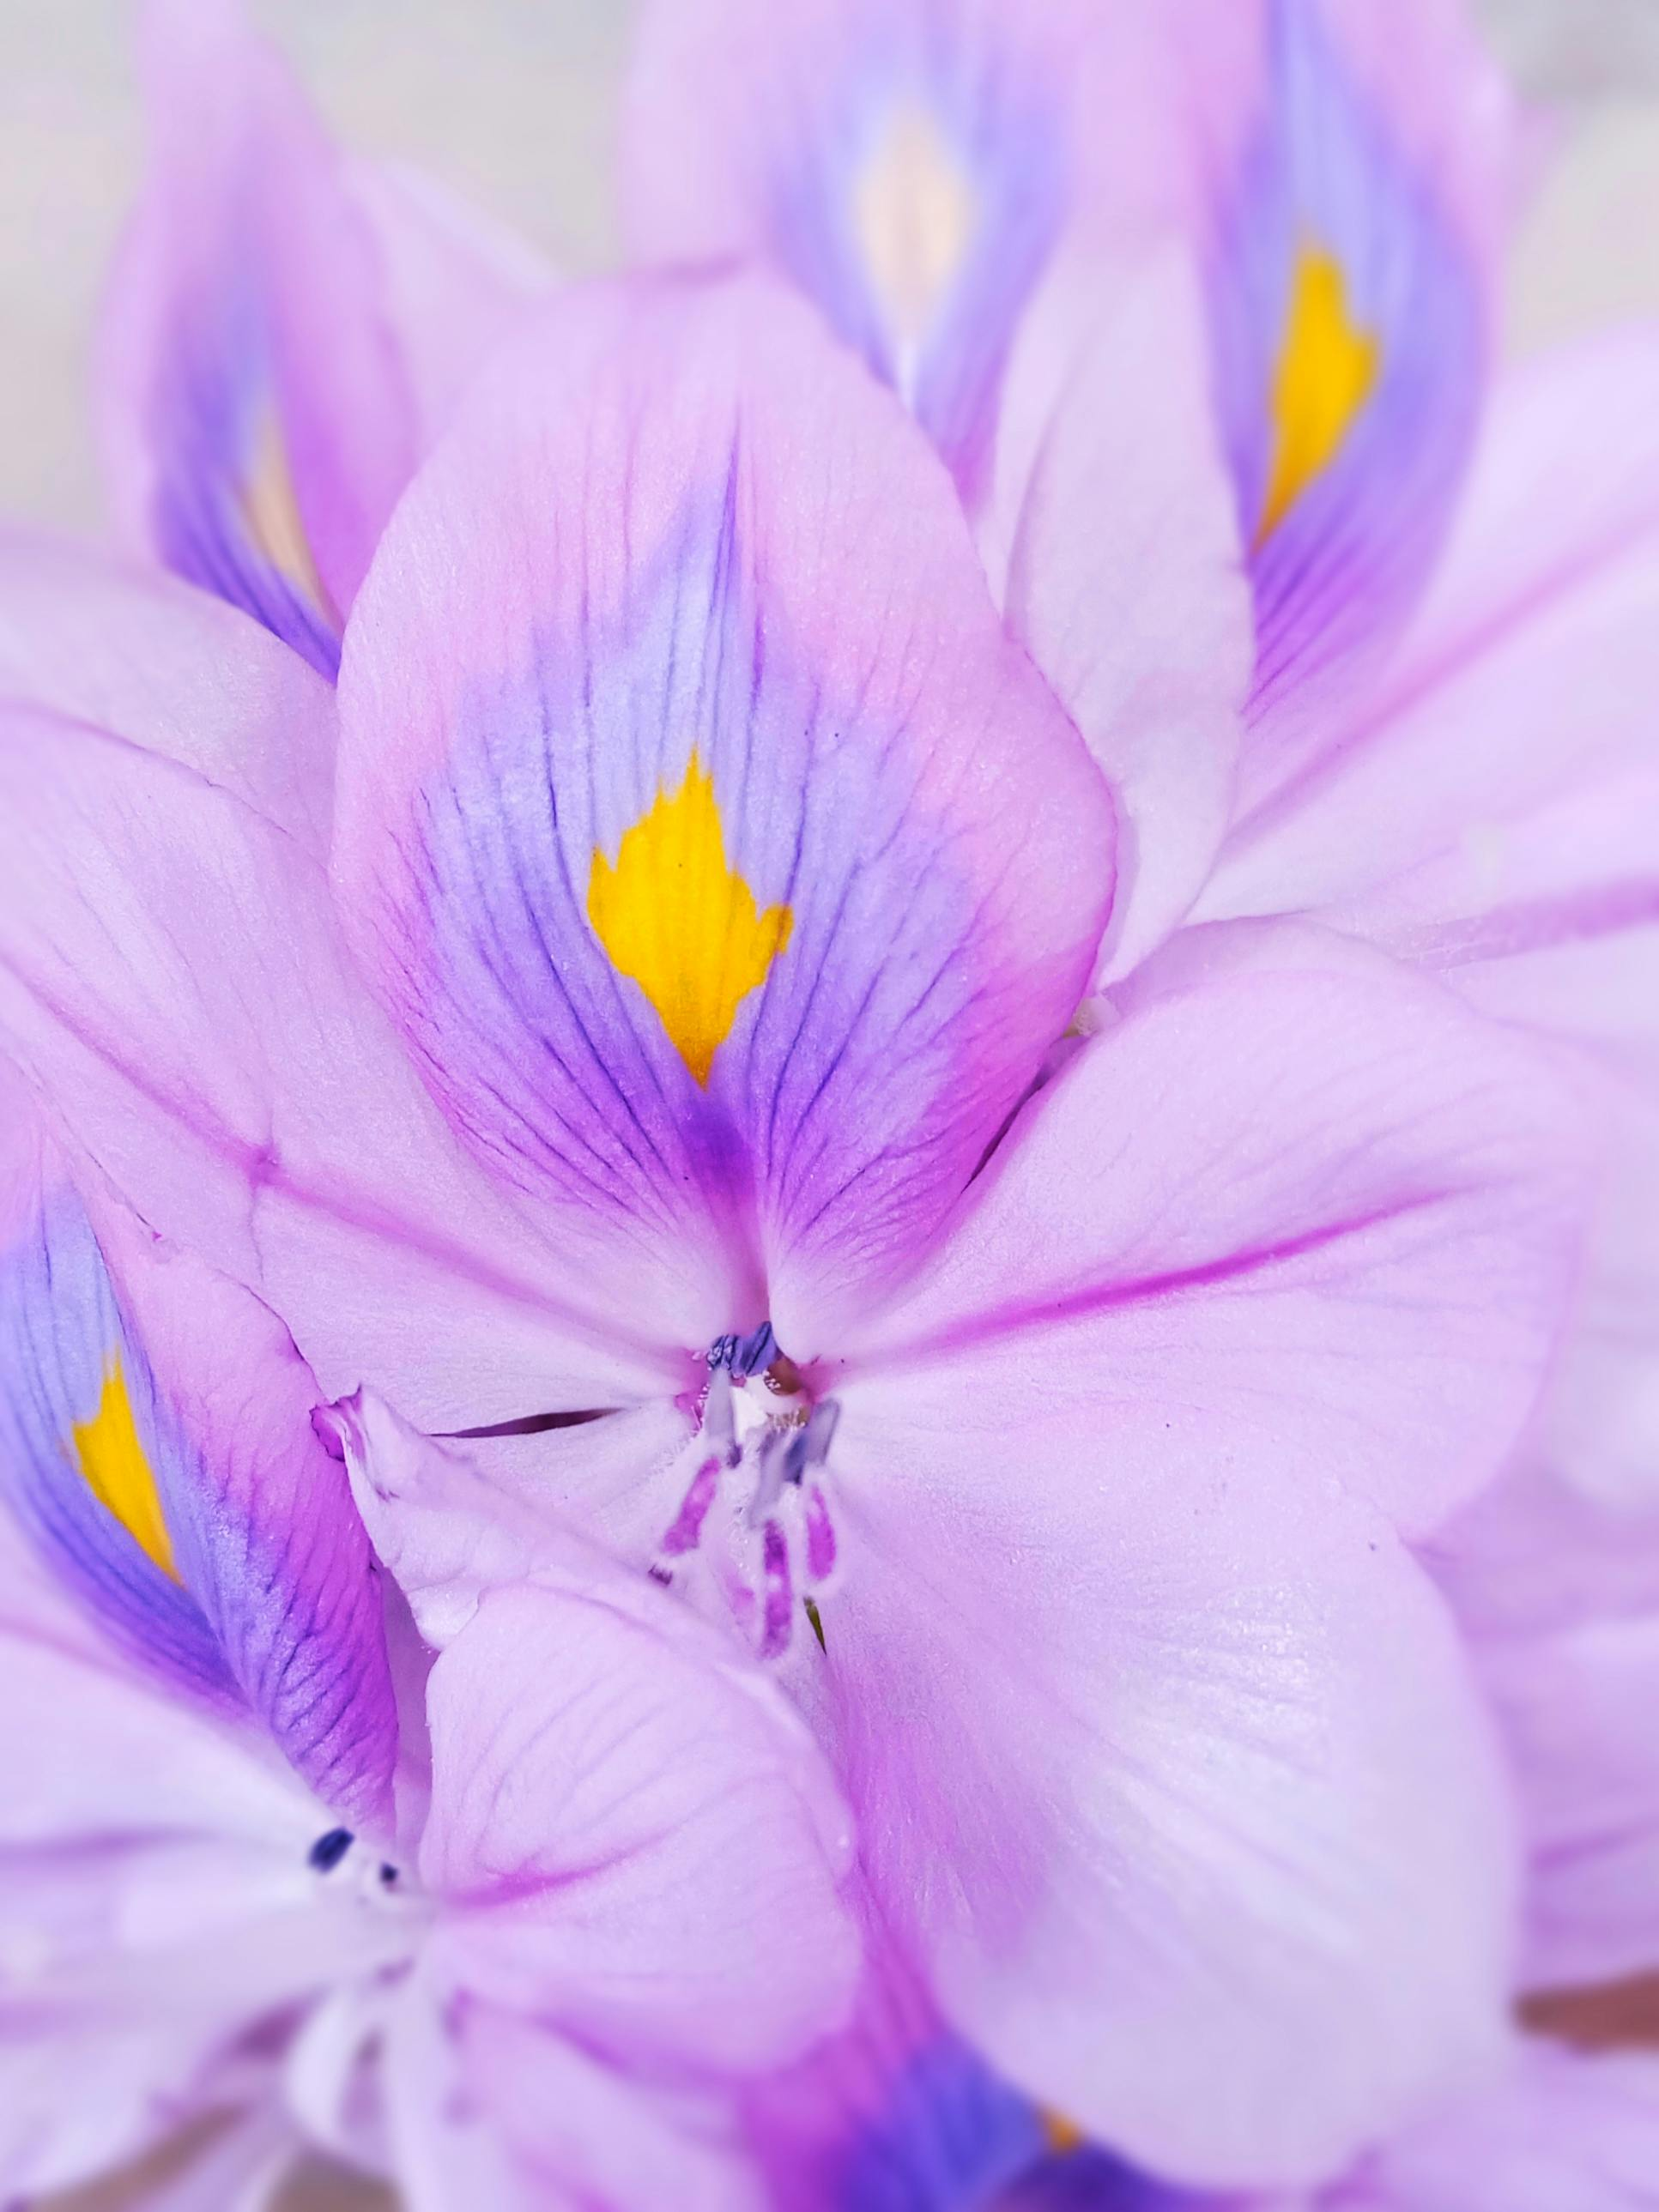
\includegraphics[height=0.85\textheight]{material/pexels-naznin-jhumur-46789485-7528634}
}}
\only<2>{\centering{
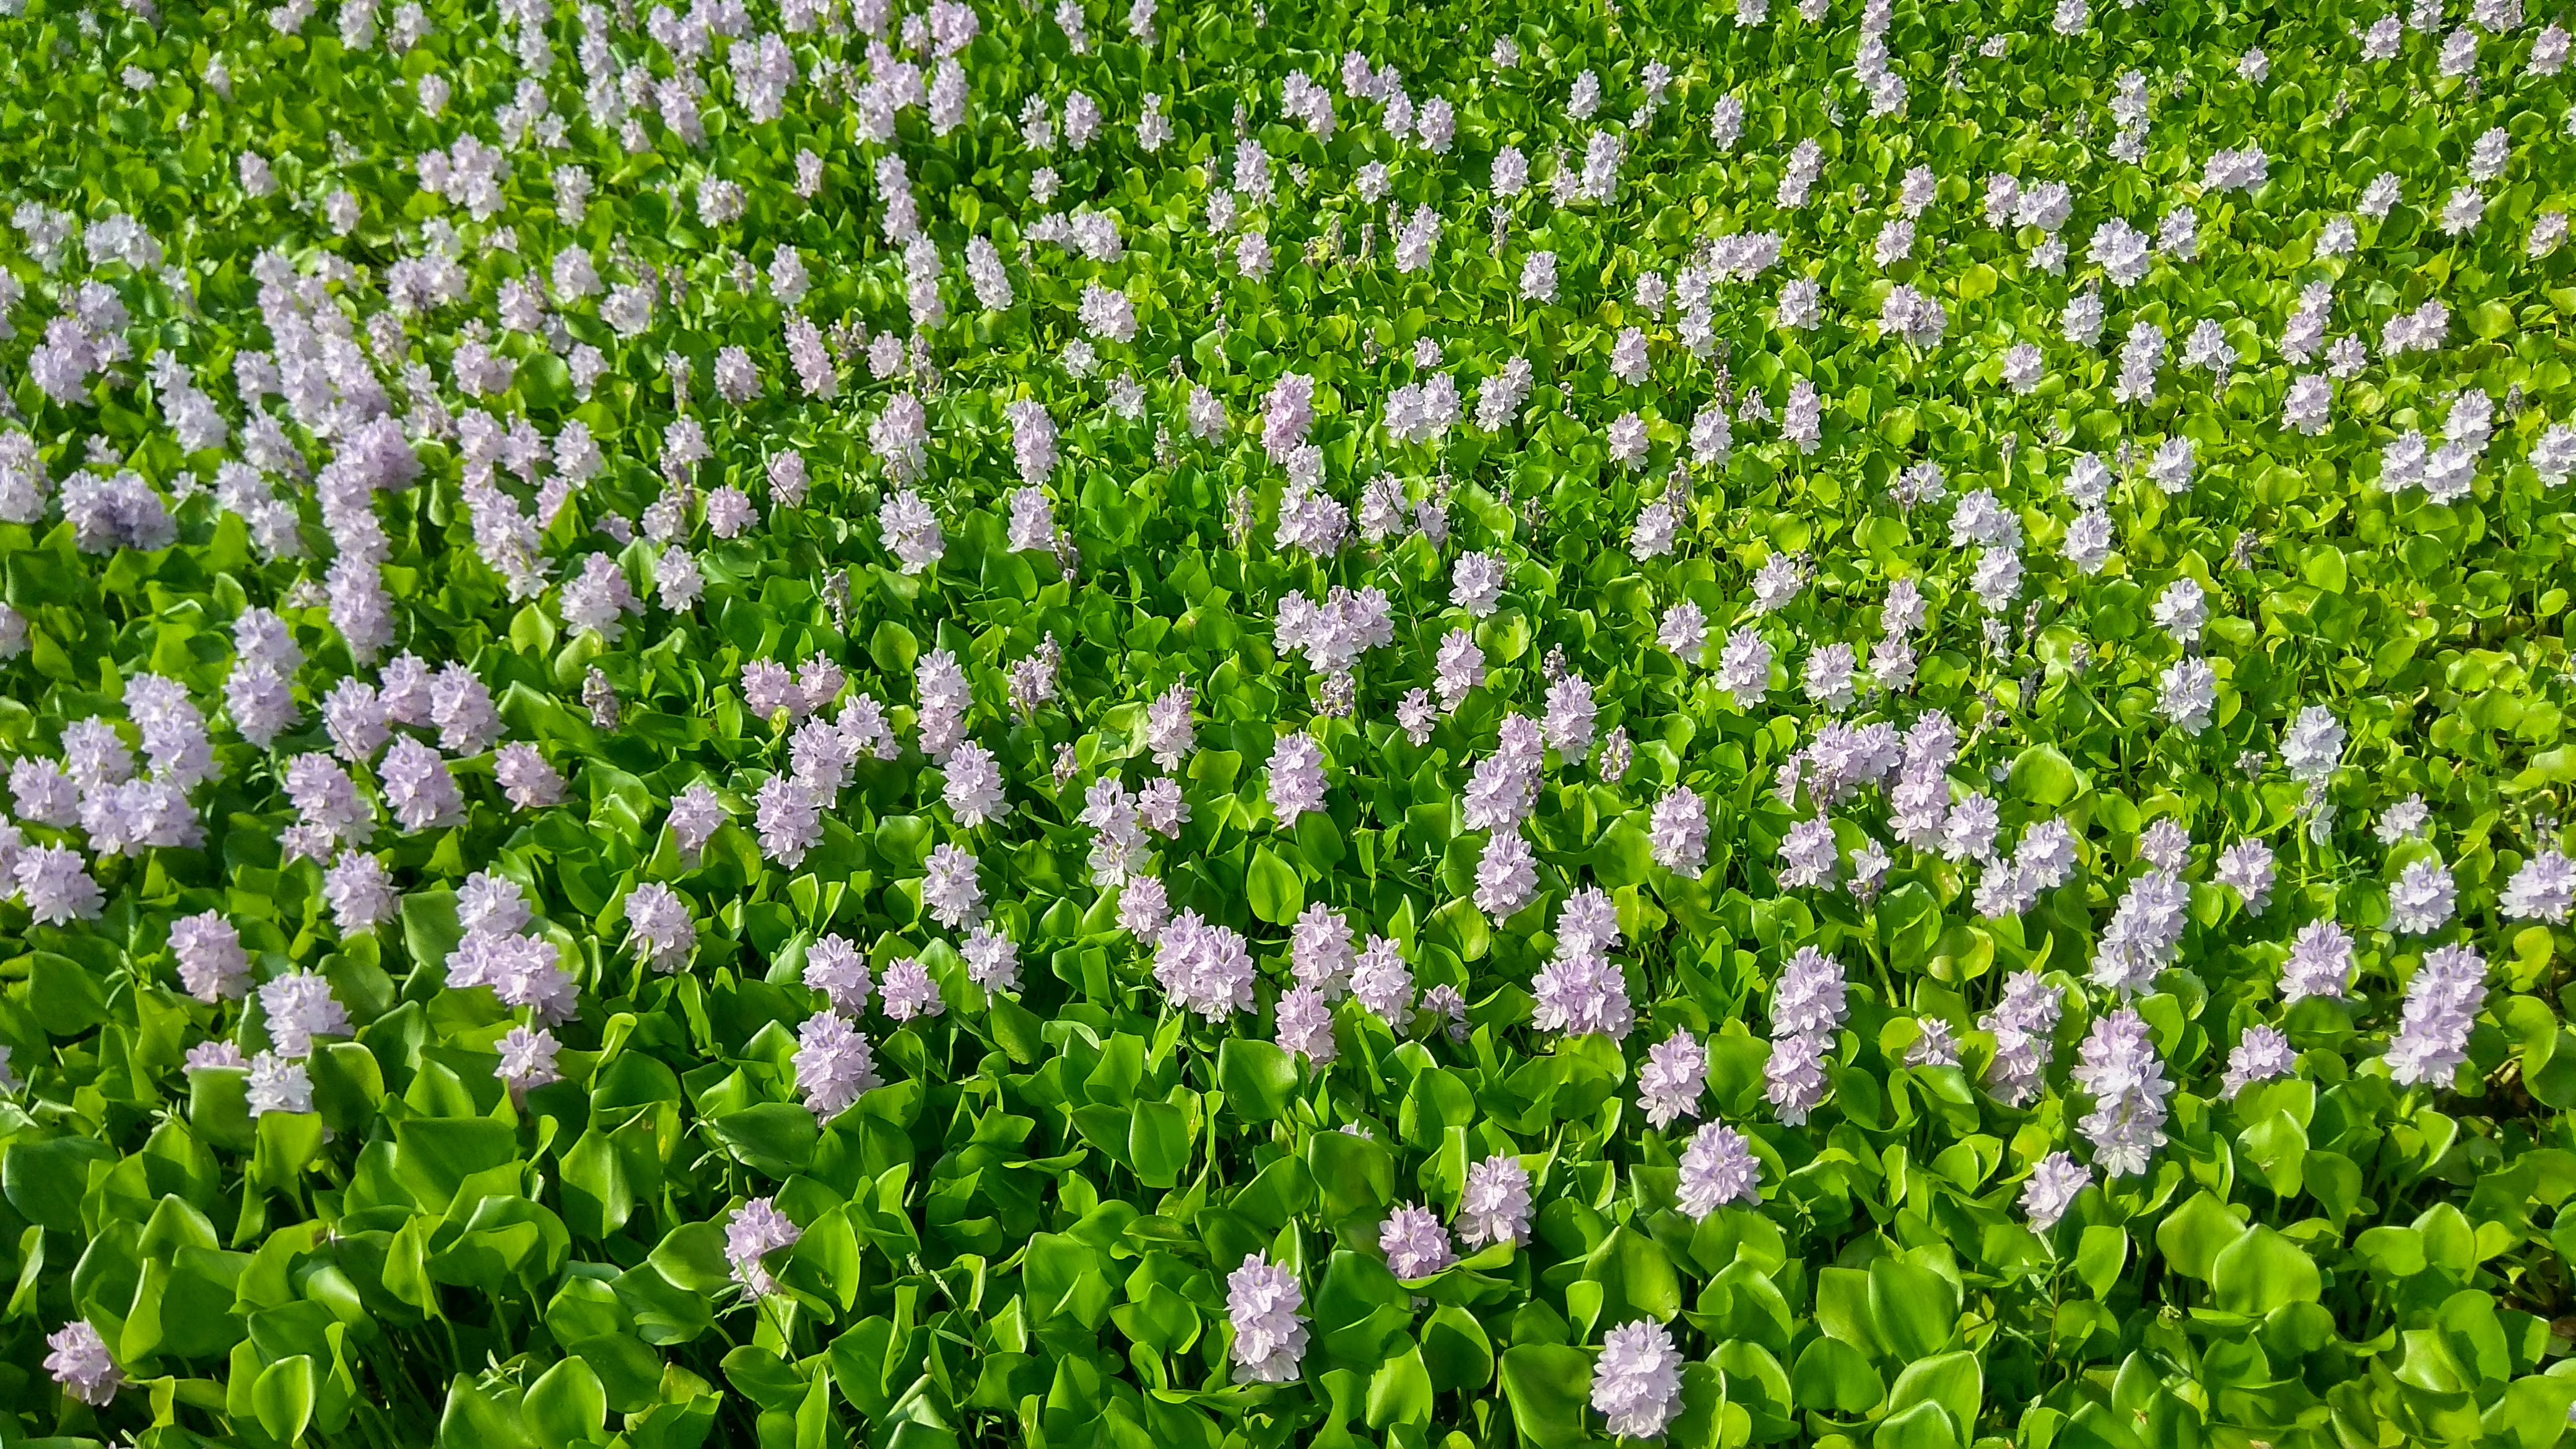
\includegraphics[height=0.85\textheight]{material/Common_Water_Hyacinth_Flower}
 }}
\end{frame}

\section[Schlüsselaspekte]{Biologische Schlüsselaspekte \& Monitoring-Relevanz (Hartbeespoort-Damm)}

% ------------------------------------------------------------
\begin{frame}{Wasserhyazinthe: Biologie \& Wirkung}
\begin{itemize}
  \item \alert{Art:} Wasserhyazinthe (\textit{Eichhornia crassipes})
  \item \alert{Wuchsform:} frei schwimmende Süßwasserpflanze, bildet dichte Oberflächenmatten
  \item \alert{Fortpflanzung:} v.\,a. vegetativ über Ausläufer (schnelle Ausbreitung), zusätzlich Samen (Persistenz)
  \item \alert{Wirkung der Matten:}
    \begin{itemize}
      \item starke \alert{Beschattung} $\rightarrow$ weniger Licht, veränderte Primärproduktion
      \item weniger \alert{Gasaustausch} $\rightarrow$ sinkender \alert{gelöster Sauerstoff} (Hypoxie/Anoxie-Risiko)
      \item Habitat- und Biodiversitätsänderungen; Störung der Ökosystemfunktion
    \end{itemize}
\end{itemize}
\end{frame}

% ------------------------------------------------------------
\begin{frame}{Warum invasiv \& was steuert die Ausbreitung?}
\begin{itemize}
  \item \alert{Invasiv, weil:}
  \begin{itemize}
    \item historische \alert{Zierpflanzen-Einfuhr} (Teich- und Wasserpflanzenhandel)
    \item hohe Wachstumsrate
    \item effiziente klonale Vermehrung
    \item wenige Gegenspieler
  \end{itemize}
  \item \alert{Begünstigt durch:} \alert{nährstoffreiche} Gewässer (Eutrophierung) und breite Umwelttoleranz
  \item \alert{Treiber der Verteilung:}
    \begin{itemize}
      \item \alert{Nitrate \& Phosphate} (Abwasser, Düngung: begünstigt Wachstum, Biomasse, Mattendicke)
      \item \alert{Wind/Strömung} (Drift, Akkumulation in Buchten/Ufernähe; Fragmentierung $\rightarrow$ neue Kolonien)
      \item \alert{Temperatur/Saisonalität} (warmes Wasser $\rightarrow$ schnelleres Wachstum)
      \item \alert{Störungen/Management} (Umlagerung, Fragmentierung)
    \end{itemize}
\end{itemize}
\end{frame}

% ------------------------------------------------------------
\begin{frame}{Monitoring \& Management: was messen, wozu?}
\begin{itemize}
  \item \alert{Kernaussage:} Wasserchemie $\rightarrow$ Wachstumspotenzial; Matten $\rightarrow$ Rückkopplung auf Licht/Sauerstoff
  \item \alert{Zentrale Messgrößen (IoT-tauglich):}
    \begin{itemize}
      \item \alert{Nährstoffe} (NO$_3^-$, NH$_4^+$, PO$_4^{3-}$) als zentrale Treiber (wo möglich/vertretbar messen)
      \item \alert{Leitfähigkeit/TDS}, \alert{pH}, \alert{Temperatur}, \alert{Trübung}, \alert{gelöster Sauerstoff}
    \end{itemize}
  \item \alert{Nutzen:} Frühwarnung, räumliches Verständnis (Zuflüsse/Buchten/Wind), Erfolgskontrolle von Maßnahmen
  \item \alert{Bekämpfung (integriert):}
    \begin{itemize}
      \item \alert{Quellenkontrolle:} Nährstoffeinträge reduzieren (langfristig entscheidend)
      \item \alert{Bio-Kontrolle} (z.\,B. Rüsselkäfer) + \alert{mechanische Entnahme} (lokal schnell, aber teuer)
      \item \alert{Chemische Mittel} nur reguliert/gezielt; immer begleitet durch Monitoring
    \end{itemize}
\end{itemize}
\end{frame}


% \section[withsectionpage][Biologische Schlüsselaspekte]{Biologische Schlüsselaspekte \& Relevanz für das Monitoring des Hartbeespoort-Damms}
%
% \begin{frame}{Art \& Grundlagenbiologie}
% \begin{itemize}
% \item \alert{Art:} Wasserhyazinthe (\textit{Eichhornia crassipes} / häufig auch \textit{Pontederia crassipes})
% \item \alert{Wuchsform:} Frei schwimmende Süßwasser-Makrophyte, die dichte Oberflächenmatten bildet
% \item \alert{Fortpflanzung:}
%     \begin{itemize}
% \item Überwiegend \alert{vegetativ} über Ausläufer (rasche klonale Ausbreitung)
% \item Auch \alert{sexuell} über Samen (längerfristige Persistenz)
%     \end{itemize}
% \item \alert{Ökologische Effekte der Matten:}
%     \begin{itemize}
% \item Starke \alert{Beschattung} $\rightarrow$ weniger Licht unter Wasser, veränderte Primärproduktion
% \item Reduzierter \alert{Gasaustausch} und \alert{gelöster Sauerstoff} (Risiko für Hypoxie/Anoxie)
% \item Habitatveränderung; Auswirkungen auf Biodiversität und Ökosystemfunktion
%     \end{itemize}
% \end{itemize}
% \end{frame}
%
% \begin{frame}{Warum sie invasiv ist (allgemeine Invasionsbiologie)}
% \begin{itemize}
% \item \alert{Außerhalb ihres natürlichen Verbreitungsgebiets eingeführt} (Südamerika) und als selbsterhaltende Population etabliert
% \item \alert{Hohe intrinsische Wachstumsrate} und effiziente vegetative Vermehrung
% \item \alert{Ökologische Entlastung:} weniger wirksame natürliche Gegenspieler (Herbivoren/Pathogene) als im Herkunftsgebiet
% \item \alert{Breite Toleranz} gegenüber Umweltbedingungen; gedeiht besonders in nährstoffreichen Gewässern
% \item \alert{Hohe Konkurrenzstärke:} rasche Oberflächenbedeckung blockiert Ressourcen (Licht/Platz/Sauerstoff)
% \end{itemize}
% \end{frame}
%
% \begin{frame}{Wie sie vermutlich eingeschleppt wurde (Südafrika / Hartbeespoort-Kontext)}
% \begin{itemize}
% \item \alert{Hauptpfad:} historische \alert{Zierpflanzen-Einfuhr} (Teich- und Wasserpflanzenhandel)
% \item \alert{Sekundäre Ausbreitung:}
%     \begin{itemize}
% \item Verschleppung von Pflanzenfragmenten zwischen Gewässern (Boote, Fischereigerät, Wasserüberleitungen)
% \item Vernetzung von Flüssen/Reservoirs ermöglicht Abdrift flussabwärts und Etablierung in geschützten Buchten
%     \end{itemize}
% \item \alert{Lokale Verstärkung in Stauseen:} Eutrophierung und stabile Oberflächenwasserbedingungen fördern den raschen Biomasseaufbau
% \end{itemize}
% \end{frame}
%
% \begin{frame}{Treiber der Ausbreitung und Verteilung (was steuert die Matten?)}
% \begin{itemize}
% \item \alert{Nährstoffverfügbarkeit (N und P):} zentraler Treiber für Wachstumsrate, Biomasse und Mattendicke
% \item \alert{Hydrodynamik:}
%     \begin{itemize}
% \item Strömungsarme / geschützte Zonen begünstigen die Etablierung (Buchten, Uferbereiche)
% \item Windgetriebene Drift aggregiert Matten; Fragmentierung ermöglicht neue Kolonien
%     \end{itemize}
% \item \alert{Klima und Saisonalität:} warme Temperaturen und hohe Einstrahlung beschleunigen das Wachstum
% \item \alert{Störungsregime:} Stürme, Hochwasser und Managementmaßnahmen können Biomasse fragmentieren und umverteilen
% \item \alert{Biotische Regulation:} Wirksamkeit von Herbivoren/Pathogenen (natürlich oder für biologische Bekämpfung eingebracht)
% \end{itemize}
% \end{frame}
%
% \begin{frame}{Warum Wasserchemie wichtig ist (und was zu beobachten ist)}
% \begin{itemize}
% \item Wasserhyazinthen werden stark durch \alert{Eutrophierung} (Nährstoffüberschuss) begünstigt
% \item \alert{Nährstoffeinträge} (Abwässer, landwirtschaftlicher Oberflächenabfluss) entscheiden häufig darüber, ob Bekämpfung nachhaltig ist
% \item \alert{Zentrale wasserchemische / physikalisch-chemische Größen:}
%     \begin{itemize}
% \item \alert{Nährstoffe:} Nitrat, Ammonium, Phosphat (oft am aussagekräftigsten)
% \item \alert{Leitfähigkeit / TDS:} Proxy für Ionenfracht; kann mit Zuflüssen und Belastung korrelieren
% \item \alert{pH:} beeinflusst Nährstoffverfügbarkeit und biologischen Stress
% \item \alert{Temperatur:} steuert Stoffwechsel- und Wachstumsraten
% \item \alert{Trübung / Secchi-Tiefe:} Lichtdurchdringung; Wechselwirkung mit Beschattung und Algen
% \item \alert{Gelöster Sauerstoff:} Indikator für Ökosystemgesundheit; sinkt unter dichten Matten
%     \end{itemize}
% \item \alert{Interpretation:} Chemie $\rightarrow$ Wachstumspotenzial; Matten $\rightarrow$ Rückkopplung auf Sauerstoff/Licht
% \end{itemize}
% \end{frame}
%
% \begin{frame}{Mögliche Bekämpfung (integriertes Management)}
% \begin{itemize}
% \item \alert{Quellenkontrolle (langfristig am wichtigsten):} Nährstoffeinträge reduzieren (Abwässer, Abfluss)
% \item \alert{Biologische Bekämpfung:}
%     \begin{itemize}
% \item Eingebrachte, spezialisierte Herbivoren (z.\,B. Rüsselkäfer) reduzieren Vitalität und Mattenbildung
% \item Wirkt am besten als dauerhafter Druck; die Wirksamkeit hängt von Klima und Nährstoffstatus ab
%     \end{itemize}
% \item \alert{Mechanische Entfernung / Ernte:}
%     \begin{itemize}
% \item Rasche lokale Entlastung; hohe Betriebskosten; Risiko der Fragmentierung bei unsachgemäßer Durchführung
% \item Erfordert eine Strategie zur Handhabung/Entsorgung (oder Nutzung) der Biomasse
%     \end{itemize}
% \item \alert{Chemische Bekämpfung (Herbizide):} kann wirksam sein, erfordert jedoch sorgfältige Regulierung, Timing und Folgenabschätzung
% \item \alert{Good Practice:} Methoden kombinieren + kontinuierliches Monitoring (Biologie + Chemie + Fernerkundung)
% \end{itemize}
% \end{frame}
%
% \begin{frame}{Kernaussage für das Monitoring des Hartbeespoort-Damms}
% \begin{itemize}
% \item Die Dynamik der Wasserhyazinthen ist stark mit \alert{nährstoffgetriebenem Wachstumspotenzial} verknüpft
% \item \alert{Wasserchemie in Echtzeit} + Tracking der Oberflächenmatten ermöglicht:
%     \begin{itemize}
% \item Frühwarnung bei Bedingungen mit hohem Wachstum
% \item Evaluation von Maßnahmen (Nährstoffreduktion / Entfernung / biologische Bekämpfung)
% \item Räumliches Verständnis: wo Matten akkumulieren und warum (Wind, Buchten, Zuflüsse)
%     \end{itemize}
% \item Nachhaltige Kontrolle erfordert \alert{die Reduktion von Nährstoffeinträgen} zusätzlich zur direkten Biomassereduktion
% \end{itemize}
% \end{frame}
